\documentclass[twoside]{book}

% Packages required by doxygen
\usepackage{fixltx2e}
\usepackage{calc}
\usepackage{doxygen}
\usepackage[export]{adjustbox} % also loads graphicx
\usepackage{graphicx}
\usepackage[utf8]{inputenc}
\usepackage{makeidx}
\usepackage{multicol}
\usepackage{multirow}
\PassOptionsToPackage{warn}{textcomp}
\usepackage{textcomp}
\usepackage[nointegrals]{wasysym}
\usepackage[table]{xcolor}

% Font selection
\usepackage[T1]{fontenc}
\usepackage[scaled=.90]{helvet}
\usepackage{courier}
\usepackage{amssymb}
\usepackage{sectsty}
\renewcommand{\familydefault}{\sfdefault}
\allsectionsfont{%
  \fontseries{bc}\selectfont%
  \color{darkgray}%
}
\renewcommand{\DoxyLabelFont}{%
  \fontseries{bc}\selectfont%
  \color{darkgray}%
}
\newcommand{\+}{\discretionary{\mbox{\scriptsize$\hookleftarrow$}}{}{}}

% Page & text layout
\usepackage{geometry}
\geometry{%
  a4paper,%
  top=2.5cm,%
  bottom=2.5cm,%
  left=2.5cm,%
  right=2.5cm%
}
\tolerance=750
\hfuzz=15pt
\hbadness=750
\setlength{\emergencystretch}{15pt}
\setlength{\parindent}{0cm}
\setlength{\parskip}{3ex plus 2ex minus 2ex}
\makeatletter
\renewcommand{\paragraph}{%
  \@startsection{paragraph}{4}{0ex}{-1.0ex}{1.0ex}{%
    \normalfont\normalsize\bfseries\SS@parafont%
  }%
}
\renewcommand{\subparagraph}{%
  \@startsection{subparagraph}{5}{0ex}{-1.0ex}{1.0ex}{%
    \normalfont\normalsize\bfseries\SS@subparafont%
  }%
}
\makeatother

% Headers & footers
\usepackage{fancyhdr}
\pagestyle{fancyplain}
\fancyhead[LE]{\fancyplain{}{\bfseries\thepage}}
\fancyhead[CE]{\fancyplain{}{}}
\fancyhead[RE]{\fancyplain{}{\bfseries\leftmark}}
\fancyhead[LO]{\fancyplain{}{\bfseries\rightmark}}
\fancyhead[CO]{\fancyplain{}{}}
\fancyhead[RO]{\fancyplain{}{\bfseries\thepage}}
\fancyfoot[LE]{\fancyplain{}{}}
\fancyfoot[CE]{\fancyplain{}{}}
\fancyfoot[RE]{\fancyplain{}{\bfseries\scriptsize Generated by Doxygen }}
\fancyfoot[LO]{\fancyplain{}{\bfseries\scriptsize Generated by Doxygen }}
\fancyfoot[CO]{\fancyplain{}{}}
\fancyfoot[RO]{\fancyplain{}{}}
\renewcommand{\footrulewidth}{0.4pt}
\renewcommand{\chaptermark}[1]{%
  \markboth{#1}{}%
}
\renewcommand{\sectionmark}[1]{%
  \markright{\thesection\ #1}%
}

% Indices & bibliography
\usepackage{natbib}
\usepackage[titles]{tocloft}
\setcounter{tocdepth}{3}
\setcounter{secnumdepth}{5}
\makeindex

% Hyperlinks (required, but should be loaded last)
\usepackage{ifpdf}
\ifpdf
  \usepackage[pdftex,pagebackref=true]{hyperref}
\else
  \usepackage[ps2pdf,pagebackref=true]{hyperref}
\fi
\hypersetup{%
  colorlinks=true,%
  linkcolor=blue,%
  citecolor=blue,%
  unicode%
}

% Custom commands
\newcommand{\clearemptydoublepage}{%
  \newpage{\pagestyle{empty}\cleardoublepage}%
}

\usepackage{caption}
\captionsetup{labelsep=space,justification=centering,font={bf},singlelinecheck=off,skip=4pt,position=top}

%===== C O N T E N T S =====

\begin{document}

% Titlepage & ToC
\hypersetup{pageanchor=false,
             bookmarksnumbered=true,
             pdfencoding=unicode
            }
\pagenumbering{alph}
\begin{titlepage}
\vspace*{7cm}
\begin{center}%
{\Large My Project }\\
\vspace*{1cm}
{\large Generated by Doxygen 1.8.13}\\
\end{center}
\end{titlepage}
\clearemptydoublepage
\pagenumbering{roman}
\tableofcontents
\clearemptydoublepage
\pagenumbering{arabic}
\hypersetup{pageanchor=true}

%--- Begin generated contents ---
\chapter{Hierarchical Index}
\section{Class Hierarchy}
This inheritance list is sorted roughly, but not completely, alphabetically\+:\begin{DoxyCompactList}
\item Callback\begin{DoxyCompactList}
\item \contentsline{section}{group10.\+Image\+Surface}{\pageref{classgroup10_1_1_image_surface}}{}
\end{DoxyCompactList}
\item \contentsline{section}{group10.\+Ruler}{\pageref{classgroup10_1_1_ruler}}{}
\item Dialog\+Fragment\begin{DoxyCompactList}
\item \contentsline{section}{group10.\+Input\+Dialog}{\pageref{classgroup10_1_1_input_dialog}}{}
\end{DoxyCompactList}
\item Surface\+View\begin{DoxyCompactList}
\item \contentsline{section}{group10.\+Image\+Surface}{\pageref{classgroup10_1_1_image_surface}}{}
\end{DoxyCompactList}
\end{DoxyCompactList}

\chapter{Class Index}
\section{Class List}
Here are the classes, structs, unions and interfaces with brief descriptions\+:\begin{DoxyCompactList}
\item\contentsline{section}{\hyperlink{classgroup10_1_1_image_surface}{group10.\+Image\+Surface} }{\pageref{classgroup10_1_1_image_surface}}{}
\item\contentsline{section}{\hyperlink{classgroup10_1_1_input_dialog}{group10.\+Input\+Dialog} }{\pageref{classgroup10_1_1_input_dialog}}{}
\item\contentsline{section}{\hyperlink{classgroup10_1_1_ruler}{group10.\+Ruler} }{\pageref{classgroup10_1_1_ruler}}{}
\end{DoxyCompactList}

\chapter{Class Documentation}
\hypertarget{classgroup10_1_1_image_surface}{}\section{group10.\+Image\+Surface Class Reference}
\label{classgroup10_1_1_image_surface}\index{group10.\+Image\+Surface@{group10.\+Image\+Surface}}
Inheritance diagram for group10.\+Image\+Surface\+:\begin{figure}[H]
\begin{center}
\leavevmode
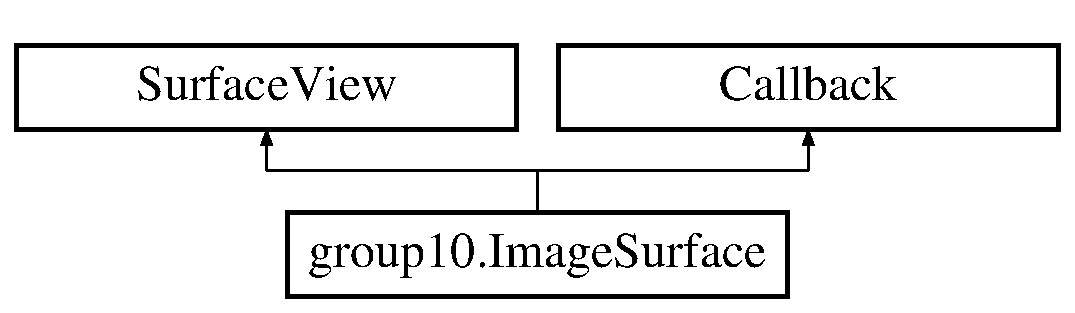
\includegraphics[height=2.000000cm]{classgroup10_1_1_image_surface}
\end{center}
\end{figure}
\subsection*{Public Member Functions}
\begin{DoxyCompactItemize}
\item 
\mbox{\Hypertarget{classgroup10_1_1_image_surface_acb219d08e16a74ff7ab58c2957c29aac}\label{classgroup10_1_1_image_surface_acb219d08e16a74ff7ab58c2957c29aac}} 
{\bfseries Image\+Surface} (Context context, File image)
\item 
\mbox{\Hypertarget{classgroup10_1_1_image_surface_a2940f5fa002d6230fb587258fb283df8}\label{classgroup10_1_1_image_surface_a2940f5fa002d6230fb587258fb283df8}} 
void {\bfseries surface\+Changed} (Surface\+Holder holder, int format, int width, int height)
\item 
\mbox{\Hypertarget{classgroup10_1_1_image_surface_a3138d80ebcd6592d39c3a772cab911a0}\label{classgroup10_1_1_image_surface_a3138d80ebcd6592d39c3a772cab911a0}} 
void {\bfseries surface\+Created} (Surface\+Holder holder)
\item 
\mbox{\Hypertarget{classgroup10_1_1_image_surface_aa7b7e12958e9fb0d40185344bb721afa}\label{classgroup10_1_1_image_surface_aa7b7e12958e9fb0d40185344bb721afa}} 
void {\bfseries surface\+Destroyed} (Surface\+Holder holder)
\end{DoxyCompactItemize}
\subsection*{Protected Member Functions}
\begin{DoxyCompactItemize}
\item 
\mbox{\Hypertarget{classgroup10_1_1_image_surface_aabe5cce015004a489330069414a9c5eb}\label{classgroup10_1_1_image_surface_aabe5cce015004a489330069414a9c5eb}} 
void {\bfseries on\+Draw} (Canvas canvas)
\end{DoxyCompactItemize}
\subsection*{Private Attributes}
\begin{DoxyCompactItemize}
\item 
\mbox{\Hypertarget{classgroup10_1_1_image_surface_aa14008274261258bdf3df75456e47c65}\label{classgroup10_1_1_image_surface_aa14008274261258bdf3df75456e47c65}} 
Bitmap {\bfseries icon}
\item 
\mbox{\Hypertarget{classgroup10_1_1_image_surface_a00b13a5d8db1f4ca0ae28f725b043145}\label{classgroup10_1_1_image_surface_a00b13a5d8db1f4ca0ae28f725b043145}} 
Paint {\bfseries paint}
\end{DoxyCompactItemize}


\subsection{Detailed Description}
Class used to handle displaying the photo/image to the user. 

The documentation for this class was generated from the following file\+:\begin{DoxyCompactItemize}
\item 
C\+:/\+Users/princ/\+Desktop/eng 3/3xa3/source/Image\+Surface.\+java\end{DoxyCompactItemize}

\hypertarget{classgroup10_1_1_input_dialog}{}\section{group10.\+Input\+Dialog Class Reference}
\label{classgroup10_1_1_input_dialog}\index{group10.\+Input\+Dialog@{group10.\+Input\+Dialog}}
Inheritance diagram for group10.\+Input\+Dialog\+:\begin{figure}[H]
\begin{center}
\leavevmode
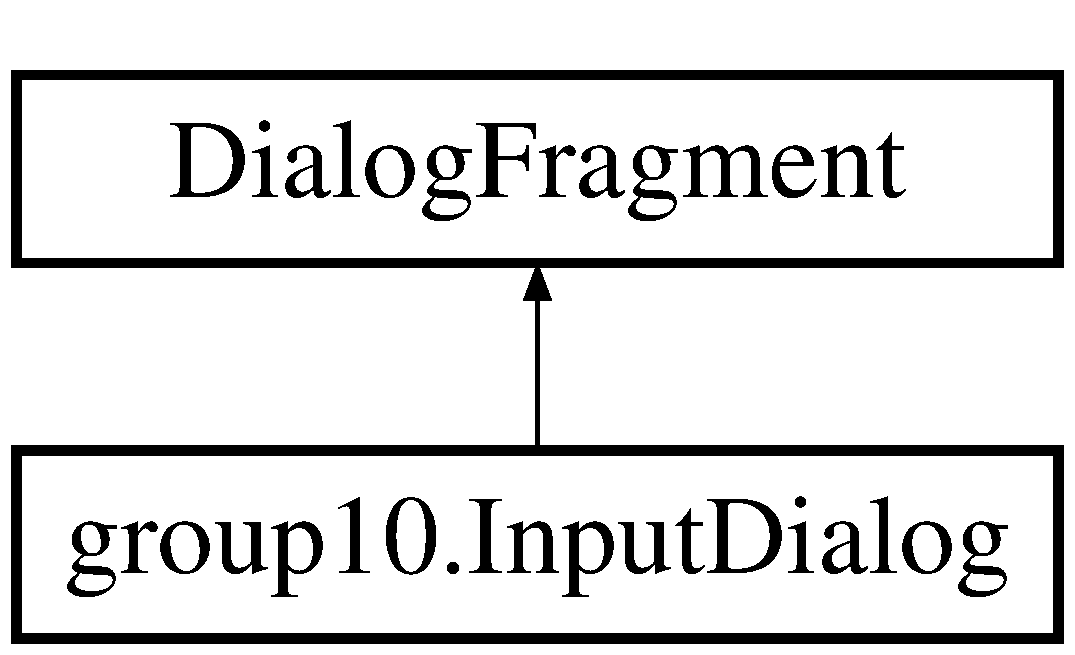
\includegraphics[height=2.000000cm]{classgroup10_1_1_input_dialog}
\end{center}
\end{figure}
\subsection*{Public Member Functions}
\begin{DoxyCompactItemize}
\item 
\mbox{\Hypertarget{classgroup10_1_1_input_dialog_a95c3498b45e142b4c20ec2a5fb8d93f1}\label{classgroup10_1_1_input_dialog_a95c3498b45e142b4c20ec2a5fb8d93f1}} 
Dialog {\bfseries on\+Create\+Dialog} (Bundle saved\+Instance\+State)
\end{DoxyCompactItemize}


The documentation for this class was generated from the following file\+:\begin{DoxyCompactItemize}
\item 
C\+:/\+Users/princ/\+Desktop/eng 3/3xa3/source/Input\+Dialog.\+java\end{DoxyCompactItemize}

\hypertarget{classgroup10_1_1_ruler}{}\section{group10.\+Ruler Class Reference}
\label{classgroup10_1_1_ruler}\index{group10.\+Ruler@{group10.\+Ruler}}
\subsection*{Static Public Member Functions}
\begin{DoxyCompactItemize}
\item 
static double \hyperlink{classgroup10_1_1_ruler_a80bd8e8dfeeb8e4160486ad01d6ca03e}{compute} (List$<$ Point $>$ points, double scale, int input\+Unit\+Index, int output\+Unit\+Index)
\end{DoxyCompactItemize}
\subsection*{Static Private Member Functions}
\begin{DoxyCompactItemize}
\item 
static double \hyperlink{classgroup10_1_1_ruler_a9dec5abc444282d874dc441fe66daa40}{get\+Distance} (Point p1, Point p2)
\item 
static double \hyperlink{classgroup10_1_1_ruler_a3447089ea321fa737049b10daaecfa0e}{convert\+Units} (int ref\+Unit, double reference, int mea\+Unit, double measurement)
\item 
static double \hyperlink{classgroup10_1_1_ruler_a23c8d18380fb06f65ee8722a355baebf}{to\+Meters} (double measurement, int ref\+Unit)
\end{DoxyCompactItemize}


\subsection{Detailed Description}
Class that handles all the mathematical operations. 

\subsection{Member Function Documentation}
\mbox{\Hypertarget{classgroup10_1_1_ruler_a80bd8e8dfeeb8e4160486ad01d6ca03e}\label{classgroup10_1_1_ruler_a80bd8e8dfeeb8e4160486ad01d6ca03e}} 
\index{group10\+::\+Ruler@{group10\+::\+Ruler}!compute@{compute}}
\index{compute@{compute}!group10\+::\+Ruler@{group10\+::\+Ruler}}
\subsubsection{\texorpdfstring{compute()}{compute()}}
{\footnotesize\ttfamily static double group10.\+Ruler.\+compute (\begin{DoxyParamCaption}\item[{List$<$ Point $>$}]{points,  }\item[{double}]{scale,  }\item[{int}]{input\+Unit\+Index,  }\item[{int}]{output\+Unit\+Index }\end{DoxyParamCaption})\hspace{0.3cm}{\ttfamily [static]}}

Based on a list of 4 points, computes the distance between the last 2 using the first 2 as a reference. 
\begin{DoxyParams}{Parameters}
{\em points} & A List of 4 points \\
\hline
{\em scale} & The value of the distance between the first 2 points \\
\hline
{\em input\+Unit\+Index} & Input unit \\
\hline
{\em output\+Unit\+Index} & Output unit \\
\hline
\end{DoxyParams}
\begin{DoxyReturn}{Returns}
The value of the distance between the last 2 points 
\end{DoxyReturn}
\mbox{\Hypertarget{classgroup10_1_1_ruler_a3447089ea321fa737049b10daaecfa0e}\label{classgroup10_1_1_ruler_a3447089ea321fa737049b10daaecfa0e}} 
\index{group10\+::\+Ruler@{group10\+::\+Ruler}!convert\+Units@{convert\+Units}}
\index{convert\+Units@{convert\+Units}!group10\+::\+Ruler@{group10\+::\+Ruler}}
\subsubsection{\texorpdfstring{convert\+Units()}{convertUnits()}}
{\footnotesize\ttfamily static double group10.\+Ruler.\+convert\+Units (\begin{DoxyParamCaption}\item[{int}]{ref\+Unit,  }\item[{double}]{reference,  }\item[{int}]{mea\+Unit,  }\item[{double}]{measurement }\end{DoxyParamCaption})\hspace{0.3cm}{\ttfamily [static]}, {\ttfamily [private]}}

Converts between units of length. 
\begin{DoxyParams}{Parameters}
{\em ref\+Unit} & The unit of the reference size \\
\hline
{\em reference} & The reference size \\
\hline
{\em mea\+Unit} & The unit of the measurement size \\
\hline
{\em measurement} & The measurement size \\
\hline
\end{DoxyParams}
\begin{DoxyReturn}{Returns}
measurement converted to ref\+Unit 
\end{DoxyReturn}
\mbox{\Hypertarget{classgroup10_1_1_ruler_a9dec5abc444282d874dc441fe66daa40}\label{classgroup10_1_1_ruler_a9dec5abc444282d874dc441fe66daa40}} 
\index{group10\+::\+Ruler@{group10\+::\+Ruler}!get\+Distance@{get\+Distance}}
\index{get\+Distance@{get\+Distance}!group10\+::\+Ruler@{group10\+::\+Ruler}}
\subsubsection{\texorpdfstring{get\+Distance()}{getDistance()}}
{\footnotesize\ttfamily static double group10.\+Ruler.\+get\+Distance (\begin{DoxyParamCaption}\item[{Point}]{p1,  }\item[{Point}]{p2 }\end{DoxyParamCaption})\hspace{0.3cm}{\ttfamily [static]}, {\ttfamily [private]}}

Get the distance between 2 points 
\begin{DoxyParams}{Parameters}
{\em p1} & First point \\
\hline
{\em p2} & Second point \\
\hline
\end{DoxyParams}
\begin{DoxyReturn}{Returns}
Distance between the 2 points 
\end{DoxyReturn}
\mbox{\Hypertarget{classgroup10_1_1_ruler_a23c8d18380fb06f65ee8722a355baebf}\label{classgroup10_1_1_ruler_a23c8d18380fb06f65ee8722a355baebf}} 
\index{group10\+::\+Ruler@{group10\+::\+Ruler}!to\+Meters@{to\+Meters}}
\index{to\+Meters@{to\+Meters}!group10\+::\+Ruler@{group10\+::\+Ruler}}
\subsubsection{\texorpdfstring{to\+Meters()}{toMeters()}}
{\footnotesize\ttfamily static double group10.\+Ruler.\+to\+Meters (\begin{DoxyParamCaption}\item[{double}]{measurement,  }\item[{int}]{ref\+Unit }\end{DoxyParamCaption})\hspace{0.3cm}{\ttfamily [static]}, {\ttfamily [private]}}

Converts a value in a given unit to meters. 
\begin{DoxyParams}{Parameters}
{\em measurement} & The length value. \\
\hline
{\em ref\+Unit} & The original unit. \\
\hline
\end{DoxyParams}
\begin{DoxyReturn}{Returns}
The length value in meters 
\end{DoxyReturn}


The documentation for this class was generated from the following file\+:\begin{DoxyCompactItemize}
\item 
C\+:/\+Users/princ/\+Desktop/eng 3/3xa3/source/Ruler.\+java\end{DoxyCompactItemize}

%--- End generated contents ---

% Index
\backmatter
\newpage
\phantomsection
\clearemptydoublepage
\addcontentsline{toc}{chapter}{Index}
\printindex

\end{document}
